
\( f(x) = \dfrac{0{,}5x^3 - 3x^2 + x + 16}{x} \).

\subsection*{1.}

Il faut calculer :
\begin{align*}
f(2) &= \dfrac{0{,}5 \times 2^3 - 3 \times 2^2 + 2 + 16}{2} \\
&= \dfrac{4 - 12 + 2 + 16}{2} = \dfrac{10}{2} = 5 \text{ (milliers d'euros)}.
\end{align*}

\subsection*{2.}

\( f \) est le quotient de deux fonctions dérivables sur \([1 \,;\, 5]\), et comme la dérivée de \( \dfrac{u}{v} \) est \( \dfrac{u' v - u v'}{v^2} \), on a :

\begin{align*}
f'(x) &= \dfrac{x \left( 1{,}5x^2 - 6x + 1 \right) - 1 \left( 0{,}5x^3 - 3x^2 + x + 16 \right)}{x^2} \\
&= \dfrac{1{,}5x^3 - 0{,}5x^3 - 6x^2 + 3x^2 + x - x - 16}{x^2} \\
&= \dfrac{x^3 - 3x^2 - 16}{x^2}.
\end{align*}

\subsection*{3.}

On a, quel que soit le réel \(x\) :
\[
(x - 4)(x^2 + x + 4) = x^3 + x^2 + 4x - 4x^2 - 4x - 16 = x^3 - 3x^2 - 16.
\]

\subsection*{4.}

D'après le résultat précédent :
\[
f'(x) = \dfrac{(x - 4)(x^2 + x + 4)}{x^2},
\]
sur \([1 \,;\, 5]\).

Comme \( x^2 > 0 \), pour \( 1 \leqslant x \leqslant 5 \), le signe de \( f'(x) \) est celui du numérateur \( (x - 4)(x^2 + x + 4) \).

Le signe de \( x - 4 \) est aisé à trouver sur \( [1 \, ; 5] \) ;

Signe du trinôme \( x^2 + x + 4 \) : on a \( \Delta = 1^2 - 4 \times 4 = -16 \).

Le trinôme n'a pas de racines, et il a le signe du coefficient de \( x^2 \), donc positif pour tout réel, donc en particulier sur \( [1 \, ; 5] \).

Finalement, le signe de \( f'(x) \) est celui de \( x - 4 \).

D'où le tableau de variations avec :
\[
f(1) = 0{,}5 - 3 + 1 + 16 = 14{,}5,
\] 
\[
f(4) = \dfrac{32 - 48 + 4 + 16}{4} = 1 \quad \text{et} \quad f(5) = \dfrac{62{,}5 - 75 + 5 + 16}{5} = \dfrac{8{,}5}{5} = 1{,}7.
\]

\begin{center}
\begin{tikzpicture}
\tkzTabInit[lgt=3.5, espcl=4]{$x$ / 1, {Signe de $f'(x)$} / 1, {$f(x)$} / 2}{${1}$, ${4}$, ${5}$}
\tkzTabLine{,-,0,+,}
\tkzTabVar{+/{$14{,}5$},-/{$1$},+/{$5$}}{/}
\end{tikzpicture}
\end{center}

\subsection*{5.}

D'après le tableau de variations précédent, le minimum de la fonction \( f \) est \( f(4) = 1 \).

Il faut donc produire 4\,000 pièces pour avoir un coût minimum de 1\,000 euros correspondant à cette production.

